% coding:utf-8

%----------------------------------------
%FOSAPHY, a LaTeX-Code for a summary of basic physics
%Copyright (C) 2013, Mario Felder

%This program is free software; you can redistribute it and/or
%modify it under the terms of the GNU General Public License
%as published by the Free Software Foundation; either version 2
%of the License, or (at your option) any later version.

%This program is distributed in the hope that it will be useful,
%but WITHOUT ANY WARRANTY; without even the implied warranty of
%MERCHANTABILITY or FITNESS FOR A PARTICULAR PURPOSE.  See the
%GNU General Public License for more details.
%----------------------------------------

\chapter{Wellen}

\boxed{\parbox{\linewidth}{
	Wellentypen:
	\begin{itemize}
		\item \textbf{Transversal:} Die Auslenkung ist veritkal oder horizontal zur Fortbewegung. z.B. Seilwelle
		\item \textbf{Longitudinal:} Die Auslenkung ist in die gleiche Richtung wie die Fortbewegung. z.B. Schallwelle in Luft
	\end{itemize}
}}
\\\\
\\
Allgemein:
\[
	f(x,0)=f^*(x) \qquad \qquad f(x,t) = f^*(x-vt)
\]
\newpage


\section{Seilwelle}
Wellengleichung:
\[\boxed{
	v^2 \pdifrac{f(x,t)}{x^2} = \pdifrac{f(x,t)}{t^2}
}\]
\\
mit der Wellengeschwindigkeit:
\[\boxed{
	v = \sqrt{\frac{F_S}{\mu}} = \sqrt{\frac{F_S}{\rho S}}
}\]
\\
\begin{footnotesize}
	$\mu$: Längendichte\\
	$S$: Seilquerschnittsfläche\\
	$\rho$: Volumendichte
\end{footnotesize}


\subsection{Freihängendes Seil}
Die Spannkraft ist an jeder Höhe $x$ unterschiedlich:
\[
	\difrac{x}{t} = v = \sqrt{\frac{F_S}{\mu}} = \sqrt{\frac{x\mu \cdot g}{\mu}} \ \Rightarrow \ t = \int_{0}^{t}\di t = \int_{0}^{L}\frac{1}{\sqrt{x \cdot g}}\di x 
\]


\section{Harmonische Wellen}
Rechts laufende Sinuswelle:
\[\boxed{
	f(x,t) = A\cos \left( \frac{2\pi}{\lambda} (x-vt)+\phi \right)
}\]
\\
\begin{footnotesize}
	Eine positive Phase $\phi$ bedeutet eine Verschiebung nach links!
\end{footnotesize}
\[\boxed{
	\omega = \frac{2\pi}{T} \qquad k = \frac{2\pi}{\lambda} \qquad v = \frac{\lambda}{T} = \frac{\omega}{k}
}\]
\\
\begin{footnotesize}
	$A$: Amplitude\\
	$\omega$: Kreisfrequenz\\
	$k$: Wellenzahl\\
	$v$: Wellengeschwindigkeit\\
	$\phi$: Phasenwinkel\\
	$T$: Periodendauer\\
	$\lambda$: Wellenlänge
\end{footnotesize}


\section{Durckwellen, Schallwellen}
Schallgeschwindigkeit in einem Fluid wie Luft oder Wasser:
\[\boxed{
	v = \sqrt{\frac{1}{\kappa \cdot \rho}}
}\]
\\
\begin{footnotesize}
	$\kappa$: Kompressibilität des Fluids ($\kappa=-\frac{1}{V} \difrac{V}{p}$)\\
\end{footnotesize}
\\
Schallgeschwindigkeit einer Kompressionswelle in einem Festkörper:
\[\boxed{
	v = \sqrt{\frac{E}{\rho}}
}\]
\\
\begin{footnotesize}
	$\rho$: Dichte\\
	$E$: Elastizitätsmodul (Hooke)\\
\end{footnotesize}
\\
\noindent
\begin{tabular}{|lc|}
\hline
\rowcolor{white}Luft  ($20^\circ C$) 		& $343 \frac{m}{s}$ \\ 
\rowcolor{lgray}Helium  ($20^\circ C$) 		& $999 \frac{m}{s}$ \\ 
\rowcolor{white}Wasserstoff  ($20^\circ C$) & $1330 \frac{m}{s}$ \\ 
\rowcolor{lgray}flüssiges Helium ($4K$) 	& $211 \frac{m}{s}$ \\ 
\rowcolor{white}Wasser  ($0^\circ C$) 		& $1402 \frac{m}{s}$ \\ 
\rowcolor{lgray}Wasser  ($20^\circ C$) 		& $1482 \frac{m}{s}$ \\ 
\rowcolor{white}Quecksilber  ($20^\circ C$) & $1451 \frac{m}{s}$ \\ 
\rowcolor{lgray}Aluminium 					& $6420 \frac{m}{s}$ \\ 
\rowcolor{white}Blei 						& $1960 \frac{m}{s}$ \\ 
\rowcolor{lgray}Stahl 						& $5941 \frac{m}{s}$ \\ 
\hline
\end{tabular} 


\section{Energiefluss}
Allgemein:
\[
	P \propto A^2
\]
\\
Leistung der flachen harmonischen Seilwelle:
\[\boxed{
	P_{Seil} = \frac12 \mu v \cdot \omega^2 A^2 = \frac12 \rho S v \omega^2 A^2
}\]
\\
\begin{footnotesize}
	$\rho$: Volumendichte\\
	$S$: Seilquerschnittsfläche\\
	$\rho \cdot S = \mu$: Längendichte
\end{footnotesize}
\\\\
Für eine harmonische Schallwelle:
\[\boxed{
	P_{Schall} = \frac12 \rho S v \omega^2 A^2 = \frac12 \frac{S}{\rho v}\hat{p}^2
}\]
\\
\begin{footnotesize}
	$A$: maximale Auslenkung der Luftteilchen\\
	$\hat{p} = \rho\omega vA$: Maximum des Schalldrucks
\end{footnotesize}


\section{Intensität $I$}
Die Intensität $I$ ist definiert als die durchschnittliche Leistung $P_{av}$ einer Welle pro Einheitsfläche, senkrecht zur Ausbreitungsrichtung:
\[
	I = \frac{P_{av}}{S}
\]
\\
\begin{footnotesize}
	$S$: Querschnittsfläche\\
\end{footnotesize}
\\\\
Intensität der harmonischen Seilwelle:
\[\boxed{
	I_{Seil} = \frac12 \rho v \omega^2 A^2
}\]
\\
Intensität der harmonischen Schallwelle:
\[\boxed{
	I_{Schall} = \frac12 \frac{\hat{p}^2}{\rho v}
}\]



\subsection{Intensität und Abstand}
Die \textbf{ebene} Welle oder der gerichtete Strahl entlang $x$ (z.B. Laserstrahl):
\[\boxed{
	I(x) = \frac{P_{av}}{S} = konst.
}\]
\\
Die \textbf{Zylinder} Welle oder Kreiswelle entlang $r$ (z.B. Säulenlautsprecher):
\[\boxed{
	I(r) = \frac{P_{av}}{S_{Zylinder}} = \frac{P_{av}}{L\cdot 2\pi r} \propto \frac{1}{r}
}\]
\\
Die Kugel Welle entlang $r$ (z.B. Punktquelle):
\[\boxed{
	I(r) = \frac{P_{av}}{S_{Kugelschale}} = \frac{P_{av}}{4\pi r^2} \propto \frac{1}{r^2}
}\]



\section{Schallpegel $L$}
Wir nehmen Lautstärke lögarithmisch wahr. Zwei Frösche hören wir nicht doppelt so laut wie einen, erst zehn Frösche.
\[\boxed{
	L = 10 \cdot \log \left( \frac{I}{I_0} \right)
}\]
\\
mit:
\[
	I_0 = 10^{-12}\ \frac{W}{m^2}
\]
\\
\[\boxed{
	\frac{I_2}{I_1} = 10^{\frac{L_2 - L_1}{10}}
}\]



\section{Doppler Effekt}
\begin{figure}[h!]
	\begin{center}
		\leavevmode
		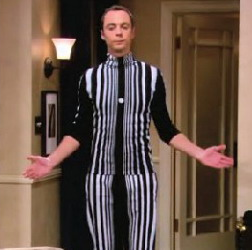
\includegraphics[scale=0.4]{../fig/dopplereffect.png}
		\caption{Why so serious?}
	\end{center}
\end{figure}
Quelle bewegt sich:
\[
	\lambda = \frac{v\mp u_s}{f_s}
\]\\
\begin{footnotesize}
	$-$: Wellenlänge vor der bewegten Quelle\\
	$+$: Wellenlänge hinter der bewegten Quelle\\
\end{footnotesize}
\\
Empfänger bewegt sich:
\[
	f_e = \frac{v \pm u_e}{\lambda}
\]\\
\begin{footnotesize}
	$+$: Bewegung zur Quelle\\
	$-$: Bewegung weg von Quelle\\
\end{footnotesize}
\\
Quelle und Empfänger bewegen sich:
\[\boxed{
	f_e = \frac{v \pm u_e}{v \mp u_s}f_s
} \qquad
	\begin{array}{l}
	+ \text{ wenn $e$ auf Quelle \textbf{zu} steuert} \\ 
	+ \text{ wenn $s$ vom Empfänger \textbf{weg} steuert}
	\end{array} 
\]
\\
\begin{footnotesize}
	$u_e$: Geschwindigkeit Empfänger\\
	$u_s$: Geschwindigkeit Sender\\
	$v$: Schallgeschwindigkeit ($343\frac{m}{s}$ @ Luft)
\end{footnotesize}



\section{Überschall}

\[\boxed{
	\sin \theta = \frac{v}{u} = \frac{1}{Ma}
}\]
\\
\begin{footnotesize}
	$\theta$: Halber Öffnungswinkel des Kegels\\
	$v$: Schallgeschwindigkeit\\
	$u$: Geschwindigkeit des Objekts\\
\end{footnotesize}


\section{Superposition - Interferenz}
\textbf{Konstruktive} Interferenz: Gleiche Phase $\Delta \phi = 0$
\[
	A = A_1 + A_2 \qquad P = \left( \sqrt{P_1} + \sqrt{P_2} \right)^2
\]
\\
\textbf{Destruktive} Interferenz: gegenphasig $\Delta \phi = \pi$
\[
	A = A_1 - A_2 \qquad P = \left( \sqrt{P_1} - \sqrt{P_2} \right)^2
\]


\section{Schwebung}
Schwebungsfrequenz:
\[\boxed{
	f_B = \frac{\Delta \omega}{2\pi} = \frac{\left| \omega_1 - \omega_2 \right|}{2\pi}
}\]
\\
Resultierende Welle:
\[
	f_{av} = \frac{\omega_1 + \omega_2}{4\pi}
\]



\section{Reflexion und Transmission}
\boxed{\parbox{\linewidth}{
	\begin{itemize}
		\item Reflexion einer Seilwelle an der Wand \textbf{invertiert} den Puls
		\item An einem losen Ende wird der Puls ohne Inversion reflektiert
		\item Trifft die Seilwelle auf ein andere Schnur, findet Reflexion und Transmission statt (Übergang leicht $\rightarrow$ schwer: invertierte Reflexion; Übergang schwer $\rightarrow$ leicht: keine Inversion)
	\end{itemize}
}}


\section{Stehende Welle}
\[\boxed{
	2A\sin(kx) \cdot \sin(\omega t)
}\]


\subsection{Harmonische}
\noindent
\begin{tabular}{|lllll|}
	\hline
	\rowcolor{white} $n$ & $\lambda$ & Bäuche & Knoten & Mitte \\
	\hline
	\rowcolor{lgray} $1$ & $\frac{2 L}{1}$ & $1$ & $2$ & Bauch \\
	\rowcolor{white} $2$ & $\frac{2 L}{2}$ & $2$ & $3$ & Knoten \\
	\rowcolor{lgray} $3$ & $\frac{2 L}{3}$ & $3$ & $4$ & Bauch \\
	\rowcolor{white} $4$ & $\frac{2 L}{4}$ & $4$ & $5$ & Knoten \\
	\rowcolor{lgray} $5$ & $\frac{2 L}{5}$ & $5$ & $6$ & Bauch \\
	\hline
\end{tabular}
\\\\\\
Eine Saite ist auf beiden Seiten eingespannt ($\Rightarrow$ Wellenknoten):
\[
	\lambda_n = \frac{2L}{n} \qquad
	f_n = \frac{v}{\lambda_n} = n \frac{v}{2L} = n \cdot f_1
\]
\\
\begin{footnotesize}
	$f_1$: Grundschwingung\\
	$n=1,2,3,\ldots$
\end{footnotesize}
\\
\[\boxed{
	y_n(x,t)=A_n \sin(k_nx) \cdot \sin(\omega_nt)
}\]
\\
\begin{footnotesize}
	$n=1$: 1. Harmonische = Grundton\\
	$n=2$: 2. Harmonische = 1. Oberschwingung\\
	$n=3$: 3. Harmonische = 2. Oberschwingung\\
\end{footnotesize}

\subsection{Orgelpfeife}
Am Ende der Pfeife ist ein Bauch:
\[
	\lambda_n = \frac{4L}{n} \qquad f_n = \frac{v}{\lambda_n} = n\frac{v}{4L} = n \cdot f_1
\]
\begin{footnotesize}
	$n=1,3,5,\ldots$
\end{footnotesize}


\subsection{Wasserwelle}
Wellengeschwindigkeit einer seichten Oberflächenwelle ($\delta y \ll y$):
\[\boxed{
	v = \sqrt{g \cdot y}
}\]
\\
Tiefwasser:
\[\boxed{
	v = \sqrt{\frac{g \lambda}{2 \pi}}
}\]
\\
\begin{footnotesize}
	$y$: Wassertiefe
\end{footnotesize}
